%!TEX root = ../Electrodynamics.tex

\subsection{\textcolor{red}{МИНИМУМ} Дисперсионное уравнение для волн в идеальной ЛП. Критические частоты и длины волн. Зависимости длины волны,
фазовой и групповой скорости от частоты. Распространяющиеся и нераспространяющиеся волны. }
Дисперсионное соотношение 
\begin{equation}
  \kappa^2 = k^2 - h^2 = \frac{\omega^2}{c^2}\epsilon\mu - h^2  
\end{equation}

\begin{figure}[h!]
  \centering
  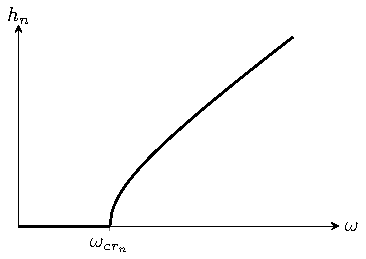
\includegraphics[scale=1.6]{img/lect2_ris6}
  \caption{Зависимость реальной части поперечного волнового числа от частоты}
  \label{fig:wavegain:5}
\end{figure}
Где $\kappa$ -- поперечное волновое число, а $h$ - продольное волновое число. 

Любая мода в линии передачи характеризуется поперечным волновым числом, а поперечное волновое число определяет продольное.

Можем ввести критическую длину волны (продольное волновое число $h$ равно нулю):
\begin{gather*}
\kappa^2 = {\frac{\omega}{c}}^2 {\epsilon \mu}\\
\omega_{cr} = \frac{\kappa c}{\sqrt{\epsilon \mu}}\\
\lambda = \frac{2 \pi c}{\omega_{cr}} = \frac{2 \pi}{\kappa \sqrt{\epsilon \mu}}
\end{gather*}
$\omega < \omega_{cr}$ дисперсионное уравнения не имеет действительных решений -- режим нераспространяющейся волны. 

При  $\omega > \omega_{cr}$ -- режим распространяющейся волны.

Если волна бежит вправо, то $h > 0$; если бежит влево, то $h < 0$

\begin{equation*}
Re{\vec{E}} , Re{\vec{H}} \sim \cos(\omega t - h z)
\end{equation*}

\begin{figure}[h!]
\centering
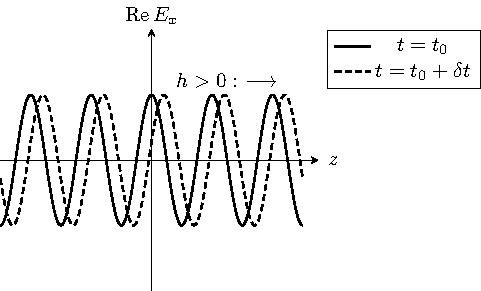
\includegraphics[scale=1]{img/lect3_ris1}
\caption{Распространение волны ($h>0$)}
\label{fig:lect3:1}
\end{figure}
При $\omega < \omega_{cr}$
\begin{equation*}
h = \pm i |h|
\end{equation*}

\begin{equation*}
Re{E_x} \sim \cos(\omega t + \phi_0) \exp{\mp |h| z}
\end{equation*}

Бегучести нет.
Зависимость экспонентальная
\begin{figure}[h!]
\centering
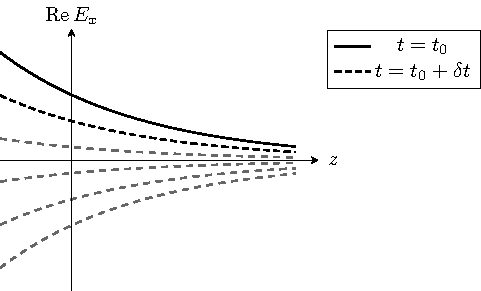
\includegraphics[scale=1]{img/lect3_ris2}
\caption{Режим нераспространения ($h<0$)}
\label{fig:lect3:2}
\end{figure}

\begin{figure}[h!]
\centering
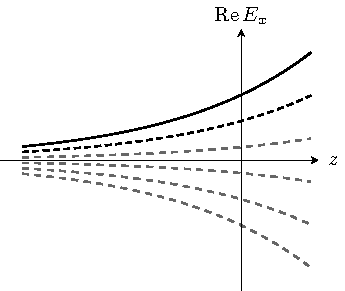
\includegraphics[scale=1]{img/lect3_ris3}
\caption{Экспоненциальное нарастание амплитуды (при $h<0$)}
\label{fig:lect3:3}
\end{figure}
Картинка зависит от способа создания волны, то есть у экспоненты << +>> или <<-->>. В зависимости от того, где источник можем сказать, куда бежит волна. То есть определить знак.

Источник может порождать несколько мод, но не все, а какие-то конкретные.
\begin{figure}[h!]
\centering
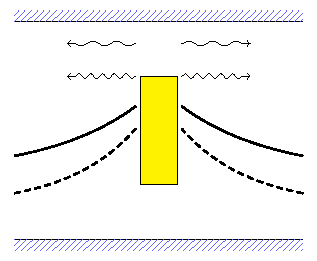
\includegraphics[scale=1]{img/lect3_ris4}
\caption{Моды в линии передачи с источником}
\label{fig:lect3:4}
\end{figure}
Изобразим числовую ось.
Пусть задана $\omega$, а то есть $k = \frac{\omega}{c} \sqrt{\epsilon \mu}$

Если $k < \kappa_1$ - все моды нераспространяющиеся.

Когда $k$ перейдёт через $\kappa_1$ появится низшая мода.

Когда перейдём через $\kappa_2$  появится ещё одна критическая частота.

!!Можно дополнить описание числовой прямой!!
\begin{figure}[h!]
\centering
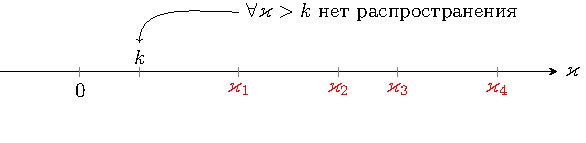
\includegraphics[scale=1]{img/lect3_ris5}
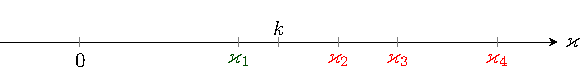
\includegraphics[scale=1]{img/lect3_ris6}
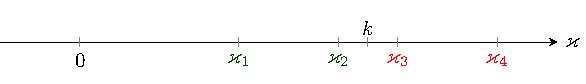
\includegraphics[scale=1]{img/lect3_ris7}
% \label{fig:lect3:4}
\end{figure}

\textbf{Кинематические соотношения} - определяют кинематические параметры волны.

\begin{enumerate}
\item Временной период 

\begin{equation*}
T = \frac{2 \pi}{\omega}
\end{equation*}

\item Длина волны в волноводе (подразумевают линию передачи или трубу, когда говорят волновод)
\begin{equation*}
\lambda_v = \frac{2 \pi}{h} = \frac{2 \pi}{\sqrt{k^2 - \kappa^2}} = \frac{2 \pi}{k} \frac{1}{\sqrt{1 - \frac{\kappa^2}{k^2}}} = \frac{\lambda_0}{\sqrt{1 - \frac{\omega_cr^2}{\omega}}} > \lambda_0
\end{equation*}

Когда $\omega \rightarrow \omega_{cr}$	$\lambda_{v} \rightarrow \infty$

$\lambda_0$ - длина волны в пространстве без волновoда в той же среде.

$\lambda_{v}$ - пространственный период.

\item Фазовая скорость - скорость перемещения плоскости постоянной фазы.

Поверхность постоянной фазы - это когда фаза константа.
\begin{equation*}
\Phi = \omega t - h z + \phi_0 = \const
\end{equation*}

При данном времени можно найти выражение для поверхности постоянной фазы:
\begin{equation*}
z = \frac{\omega t  + \phi_0}{ h }
\end{equation*}

Координата будет перемещаться со скоростью:
\begin{equation*}
v_f = \frac{\omega}{h}
\end{equation*}
\begin{equation*}
v_f = 
\frac{\omega}{\sqrt{k^2 - \kappa^2}} = 
\frac{\omega}{k} \frac{1}{\sqrt{1 - {\frac{k}{\kappa}^2}}} = \frac{\omega}{k} \frac{1}{\sqrt{1 - {\frac{\omega_{cr}}{\omega}^2}}} > v_f^{(0)}
\end{equation*}
\begin{equation*}
v_f^{(0)} = \frac{c}{\varepsilon \mu} = \frac{\omega}{k}
\end{equation*}
Фазовая скорость может быть больше скорости света.

\item Групповая скорость - скорость перемещения квазимонохроматического волнового пакета. 	
\begin{figure}[h!]
  \centering
  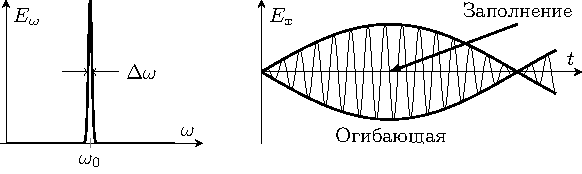
\includegraphics[scale=1]{img/lect3_ris8}
  \caption{Квазимонохроматический волновой пакет}
  \label{fig:lect3:8}
\end{figure}

Сигнал характеризуется высокочастотным заполнением и огибающей.

%	\begin{figure}[h!]
%		\centering
%		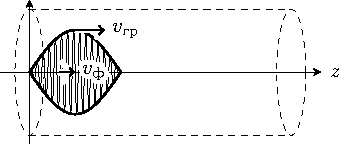
\includegraphics[scale=1]{img/lect3_ris9}
%		\caption{Распространение волнового пакета}
%		\label{fig:lect3:9}
%	\end{figure}
По сути это радиоимпульс.

Пакет движется со скоростью $ v_{gr} = \pdv{\omega}{k}\vert_{\omega = \omega_{0}} $ - это при малом или отсутствующем поглощении.(Это в пространстве, а не в линии передачи).
При большом поглощении это понятие теряет смысл. По мере перемещения по волноводу форма сигнала будет меняться.

$v_{gr} = \pdv{\omega}{h}\vert_{\omega = \omega_{0}} $ - формула для волновода. 

\begin{gather}
k^2 = h^2 + \kappa^2\\
%
k = \frac{\omega}{c} \sqrt{ \varepsilon \mu}
\end{gather}

Берём дифференциал от правой и левой части.$\kappa$  не зависит от частоты.
\begin{gather*}
2k dk = 2h dh\\
\pdv{\omega}{h} = \frac{c}{\sqrt{\varepsilon \mu}} \frac{h}{k}\\
h = + \sqrt{\frac{\omega^2}{c^2} \varepsilon \mu -\kappa^2_n}\\
\pdv{\omega}{h} = \frac{c}{\sqrt{\varepsilon \mu}} \frac{c}{\omega \sqrt{\varepsilon \mu}} \sqrt{\frac{\omega^2}{c^2} \varepsilon \mu -\kappa^2_n} = \frac{{v_f^{(0)}}^2}{v_f}
\end{gather*}

\begin{gather*}
v_{f} = \frac{\omega}{h}\\
v_{f}^{(0)} = \frac{c}{\omega \sqrt{\varepsilon \mu}}\\
%
v_{f} v_{gr} = {v_f^{(0)}}^2
\end{gather*}
\begin{equation*}
v_{gr} = v_{f}^{(0)} \sqrt{1 - {\frac{\omega_{cr}}{\omega}^2}}
\end{equation*}

Всё это справедливо для сред без временной дисперсии.
\begin{equation*}
\varepsilon\ne f(\omega), \mu \ne f(\omega)
\end{equation*}



$v_{gr} < c$ - она несёт информацию.
\end{enumerate}
\begin{figure}[h!]
\centering
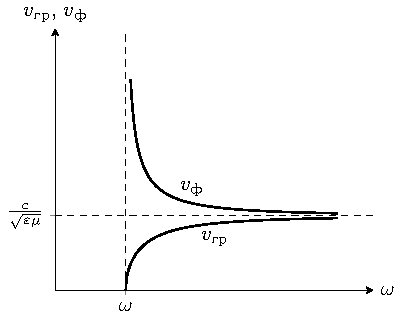
\includegraphics[scale=1]{img/lect3_ris10}
\caption{Распространение волнового пакета}
\label{fig:lect3:10}
\end{figure}
